\subsection{Data Dependencies in PDF Parsing (the Trust Chain)}
\label{sec:trust-chain}

\begin{figure}[t]
  \centering
  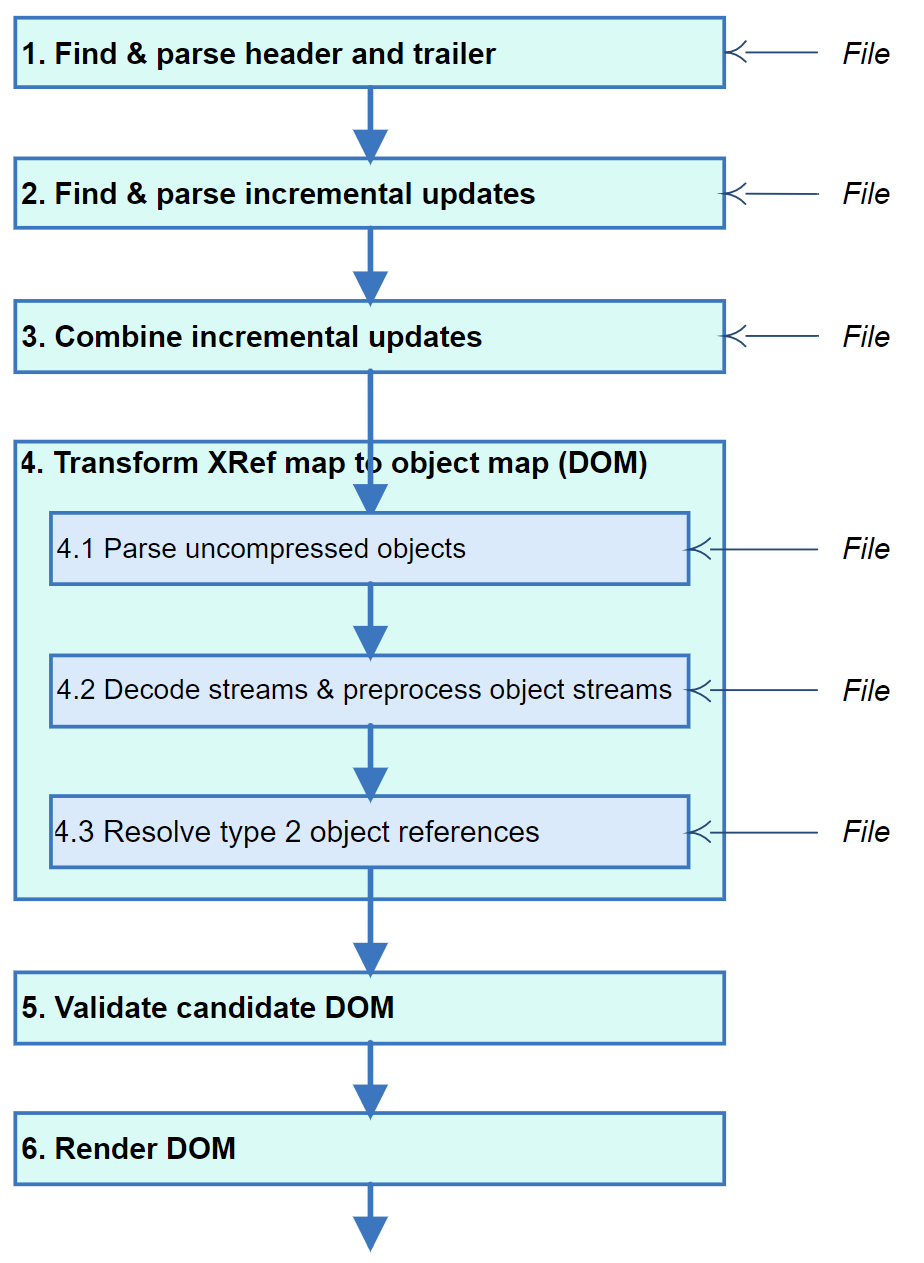
\includegraphics[width=0.8\linewidth]{figures/Stages.png}
  \caption{Stages of PDF Parsing (the Trust Chain)}
  \label{fig:pdf-trust-chain}
\end{figure}

We have touched upon the complexities of parsing
PDF, but to appreciate these, one has to understand the
dependencies and interactions between the features.
\cref{fig:pdf-trust-chain} illustrates the main stages diagrammatically:

\begin{itemize}
\item \textbf{Stage 1}: Find and parse both the PDF header and the PDF trailer to locate
  the document trailer dictionary and the start of the \emph{last} incremental update, or
  the cross reference table of the original document in the case of no updates.
\item \textbf{Stage 2}: Find and parse each cross reference table or incremental update. 
  Note that this stage uses context from Stage 1 (such as the file offset and trailer
  information) in order to know \emph{where} and \emph{how} to parse.
\item \textbf{Stage 3}: This stage computes the
   XRef map of the final PDF by accounting for each set of edits performed by each incremental update.
   Incremental updates can add new objects, mark as free previous objects, re-instate previously 
   freed objects, and change context information in the trailer dictionary that 
   forms part of each incremental update.
   Depending on the laziness of stage 2, this stage may need to do further
   parsing of the input file.
\item \textbf{Stage 4}: Transform the XRef map to an object map. This stage is complex and
  requires three sub-stages, each of which does further file input and parsing.
  Further details are in \cref{sec:specifying}.
  If all goes well, we have a syntactically valid candidate DOM.
\item \textbf{Stage 5}: Validate candidate DOM.  This stage takes the candidate DOM and
  \emph{semantically} verifies that it represents a valid document graph as per
  the PDF standard.
  %
  The candidate DOM consists of a mapping of object references to
  syntactically valid PDF objects.  
  Only at this point can we start the semantic checks such as
  dictionaries having the correct keys,
  keys having values of the expected types,
  text stream objects are syntactically valid,
  no unexpected recursion, no unresolvable object references,
  and etc.
\item \textbf{Stage 6}: Render the validated DOM. Here the validated DOM, or parts thereof, is rendered
  to the output format of choice.
\end{itemize}

Any error (malicious or otherwise) in earlier stages can affect the output of stages that follow.
Note that stages 2, 3, 4.1, 4.2, and 4.3 all depend on inputs from previous stages to determine 
where and how to parse segments of the PDF input file.
Errors that percolate into these stages can
cause all forms of havoc (parsing wrong or out-dated data, etc.).

An implementation \emph{might} merge stages 2, 3, 4.1, 4.2, 4.3 into
a single stage and give a \emph{semblance} of simplicity.
%
Our argument in what follows---particularly in
\cref{sec:single-pass-problems}---is
that such an implementation will be overly
complex and result in a design for which it is difficult
to determine if it correctly implements the standard
and to determine that it terminates for all input files.

\todo{cut the following down?: I think this is an important justification for why we don't need to address stages 5 & 6. If we remove I suspect people would say why aren't stages 5 & 6 important!}
Although \emph{Validate candidate DOM} (stage 5) might be considered tedious, the necessary checks are 
reasonably well defined by the bulk of the PDF standard. Validation involves ensuring that each 
individual PDF object has all the required keys and appropriate values in the context of its reference in the DOM.
For example, a PDF object that is a thumbnail for a PDF page needs to be an Image XObject and have a 
minimum set of required key names and their values each within predefined limits (e.g. both
\lstcd{Height} and \lstcd{Width} are required keys and must be non-negative integers). If the 
thumbnail reference in the candidate DOM is to a font dictionary or some other kind of
\emph{syntactically} valid PDF object then this is \emph{semantically} incorrect. Recent work~
\cite{peterwyattArlingtonPDFModel2021} created the first specification-derived comprehensive
machine-readable model of every object, their attributes and relationships in the PDF DOM. The use
of such a model for code generation, DOM validation, or test case generation can significantly reduce the tediousness.
\emph{Render DOM} (stage 6) also has many complications of its own,
whether this be rendering a PDF
page to pixels for display or print, or extracting text contract.

In this paper we do not further consider stages 5 and 6 but
focus on stages 1 to 4, referred to as \emph{pre-DOM} parsing or computation.
%
Errors in these stages can compromise the correctness of the complete format
definition, even if later stages are defined as intended when viewed in
isolation.

%%%%%%%%%%%%%

The term \emph{Trust Chain} (or ``Chain of Trust'') is
overloaded with similar meanings in different contexts
\begin{quote}
e.g.,
\emph{digital certificates}: a sequence of certificates signing certificates,
starting with a root certificate;
\emph{supply chain}: a product is no more reliable or secure than its
outsourced components;
\emph{trusted boot}: unless the bootloader is correct and non-malicious,
there can be no possibility of the operating system being the same;
\emph{software stacks}: upper layers are dependent upon lower layers (such as
system libraries) and vulnerabilities at the lower layers affect all higher
layers,
\end{quote}
but the common idea is that we have layers (or components)
that rely on lower layers (sub-components) for their validity.
In other words,
{\bf{A flaw in one layer of the trust chain
     causes every higher layer to be untrustworthy!}}

%%%%%%%%%%%%%

Whether or not one likes our adoption of this term,
we think it is important to understand PDF parsing in terms of the
\emph{Trust Chain} principle because
%
(1) it highlights the presence of the many ``dependent'' stages
in PDF processing;
%
(2) it highlights the importance of ensuring the pre-DOM parsing, data integrity relationships and
computation (the base of our Trust Chain) is correct and secure;
%
(3) it reminds us that the integrity of the DOM cannot be verified
independently of verifying all earlier stages; and
%
(4) it illustrates that PDF parsing, although uniquely complex, is an instance of
a general concept.

